%\documentclass[1p]{elsarticle}
\documentclass[review]{elsarticle}

\usepackage{lineno,hyperref}
\modulolinenumbers[5]

\journal{Computers \& Mathematics with Applications}

%%%%%%%%%%%%%%%%%%%%%%%
%% `Elsevier LaTeX' style
\bibliographystyle{elsarticle-num}
%%%%%%%%%%%%%%%%%%%%%%%

\usepackage{graphicx}
\usepackage{amsmath}
%\usepackage{amsfonts}
\usepackage{amssymb}
\usepackage{color}
%\usepackage{float}
\usepackage{mathtools}
\usepackage{verbatim}

\newcommand{\pdv}[2]{\frac{\partial{#1}}{\partial{#2}}}
\newcommand{\fp}[2]{\pdv{#1}{#2}}
\newcommand{\pdwc}[3]{\left(\fp{#1}{#2}\right)_{#3}}
%\newcommand{\ppdv}[3]{\displaystyle \frac{\partial^2 #1}{\partial #2\partial #3}}
\newcommand{\ppdv}[3]{\frac{\partial^2 #1}{\partial #2\partial #3}}
\newcommand{\oover}[1]{\ensuremath{\frac{1}{#1}}}

\newcommand{\vect}[1]{\boldsymbol{#1}}
\newcommand{\matr}[1]{\mathbf{#1}}
\newcommand{\dI}{\text{d}}
\newcommand{\odv}[2]{\frac{\dI #1}{\dI #2}}
\newcommand{\ddv}[2]{\odv{#1}{#2}}
%\newcommand{\ddv}[2]{\frac{\Delta #1}{\Delta #2}}
\newcommand{\mfp}{\lambda}
\newcommand{\tmfp}{\tilde{\lambda}}
\newcommand{\nue}{\nu_{e}}
\newcommand{\nutot}{\nu_{t}}
\newcommand{\vmag}{v}
\newcommand{\vth}{v_{th}}
\newcommand{\vn}{\vect{n}}
\newcommand{\E}{\vect{E}}
\newcommand{\B}{\vect{B}}
\newcommand{\tE}{\vect{\tilde{E}}}
\newcommand{\tB}{\vect{\tilde{B}}}
\newcommand{\qe}{q_e}
\newcommand{\me}{m_e}
\newcommand{\kB}{k_B}
\newcommand{\crs}{\sigma}
\newcommand{\fM}{f_M}
\newcommand{\fzero}{f_0}
\newcommand{\vfzero}{\vect{f}_0}
\newcommand{\fone}{\vect{f}_1}
\newcommand{\SM}{\vect{S}_M}
\newcommand{\MI}{\matr{I}}
\newcommand{\MA}{\matr{A}}
\newcommand{\intO}{\int_{\Omega}}
\newcommand{\IM}{\boldsymbol{\mathcal{M}}}
\newcommand{\ID}{\boldsymbol{\mathcal{D}}}
\newcommand{\IV}{\boldsymbol{\mathcal{V}}}
\newcommand{\IB}{\boldsymbol{\mathcal{B}}}
\newcommand{\anisomega}{\fone/\fzero}
\newcommand{\acl}{\vect{M}_{\left(\anisomega\right)}}

\newcommand{\figref}[1]{FIG.~\ref{#1}}
\renewcommand{\refeq}[1]{(\ref{#1})}

%%\renewcommand{\floatpagefraction}{.9}% 
%\newlength{\picwidth}
%\setlength{\picwidth}{0.49\linewidth}
%%\setlength{\picwidth}{11cm}

%%%%%%%%%%%%%%%%%%%%%%%
\begin{document}

\begin{frontmatter}

\title{High-order finite element modeling of M1-AWBS nonlocal electron transport}
%\tnotetext[mytitlenote]{}

\author[celiaaddress]{Milan, Vladimir, Philippe, Jean-Luc}
\address[celiaaddress]{Universit\'{e} de Bordeaux - CNRS - CEA, CELIA, UMR 5107, F-33405 Talence, France}


\begin{abstract}

\end{abstract}

\begin{keyword}
Nonlocal transport \sep Kinetics \sep MHD \sep High-order methods \sep FEM
%\MSC[2010] 00-01\sep  99-00
\end{keyword}

\end{frontmatter}

\linenumbers

%---------------------------------------------------------------------
%---------------------------------------------------------------------

\fbox{\parbox{0.99\textwidth}{
%\centerline{\textcolor{red}{THIS WILL BE REMOVED}}
\footnotesize
\tableofcontents
}}
\newpage

%---------------------------------------------------------------------
%---------------------------------------------------------------------
%\section{Moments method}\label{sec:moment_method}

\section{M1 model}\label{sec:m1_model}
\subsection{AWBS Boltzmann transport equation}
Simplified Boltzmann transport equation of electrons relying on the use of AWBS
collision-thermalization operator \cite{AWBS_PRL1986} reads
\begin{equation}
  \vmag\vn\cdot\nabla f + \frac{\qe}{\me}\left( \E + 
  \frac{\vmag}{c}\vn\times\B\right)\cdot\nabla_{\vect{v}} f = \nue \vmag 
  \pdv{}{\vmag}\left( f - \fM\right) .
  \label{eq:AWBS}
\end{equation}
\subsection{M1-AWBS model}
In order to eliminate the~dimensions of the~transport problem \refeq{eq:AWBS}
the~two moment model referred to as \textit{M1-AWBS} is introduced
\begin{eqnarray}
  \nue\vmag\pdv{}{\vmag}\left(\fzero - \fM \right) &=&
  \vmag\nabla\cdot\fone + \frac{\qe}{\me\vmag^2}\E\cdot\pdv{}{\vmag}
  \left( \vmag^2 \fone\right) , 
  \label{eq:M1f0}\\
  \nue\vmag\pdv{}{\vmag}\fone - \nutot\fone &=& 
  \vmag\nabla\cdot\left(\MA\fzero\right) + 
  \frac{\qe}{\me\vmag^2}\E\cdot\pdv{}{\vmag}
  \left( \vmag^2 \MA\fzero\right) \nonumber\\
  && + \frac{\qe}{\me\vmag}\E\cdot\left( \MA - \MI \right)\fzero +
  \frac{\qe}{\me c}\B\times\fone ,
  \label{eq:M1f1}
\end{eqnarray}
where the~anisotropy-closure matrix takes the~form
\begin{equation}
  \MA = \frac{1}{3}\MI + \frac{|\fone|^2}{2\fzero^2}
  \left( 1 + \frac{|\fone|^2}{\fzero^2} \right)
  \left( \frac{\fone\otimes\fone^T}{|\fone|^2} - \frac{1}{3}\MI\right) ,
\end{equation}
which corresponds to the~distribution function approximation
\begin{equation}
  f = \fzero \frac{\left|\acl\right|}{4\pi\sinh\left(\acl\right)}
  \exp\left(\vn\cdot\acl\right) ,
\end{equation}
where $\acl \rightarrow 0$ when $\anisomega \rightarrow \vect{0}$. 

%---------------------------------------------------------------------
\section{High-order finite element scheme}\label{sec:hos}
\begin{comment}
\begin{eqnarray}
  \rho \pdv{\fzero}{\vmag} &=& 
  \frac{\rho}{\nue}\MI:\nabla\fone + 
  \frac{\qe\rho}{\me\nue\vmag}\E\cdot\pdv{\fone}{\vmag}
  + \frac{2 \qe\rho}{\me\nue\vmag^2}\E\cdot\fone + \rho \pdv{\fM}{\vmag} , 
  \label{eq:M1hosf0}\\
  \rho \pdv{\fone}{\vmag} &=&
  %\frac{\rho}{\nue}\nabla\cdot\left(\MA\fzero\right) + 
  \nabla\cdot\left(\frac{\rho\MA}{\nue}\fzero\right) +
  \left(\frac{\qe\rho}{\me\nue\vmag^2}\E\cdot\left( 3\MA - \MI \right) - 
  \nabla\left( \frac{\rho}{\nue}\right)\cdot\MA \right)\fzero \nonumber\\
  &&+ \frac{\qe\rho}{\me\nue\vmag}\E\cdot\pdv{}{\vmag}
  \left( \MA\fzero\right) + \frac{\qe\rho}{\me c \nue\vmag}\B\times\fone + 
  \frac{\rho \nutot}{\nue\vmag}\fone .
  \label{eq:M1hosf1}
\end{eqnarray}
\end{comment}
\subsection{Variational principle}
First, the~electro-magnetic scaling
\begin{equation}
  \tE = \frac{\qe}{\me}\E,~\tB = \frac{\qe}{\me c} \B,
\end{equation}
is defined in order to make the~algebraic operations easier to follow.
The~general variational formulation of \eqref{eq:M1f0} and \eqref{eq:M1f1} 
constructed above the~scalar (zero moment) functional space
represented by test functions $\phi$ and the~vector
(first moment) functional space represented by test functions $\vect{w}$ 
takes the~form
\begin{eqnarray}
  \intO\phi\nue\pdv{\fzero}{\vmag} &=& 
  \intO\phi
  \left(\MI:\nabla\fone + 
  \frac{1}{\vmag}\tE\cdot\pdv{\fone}{\vmag}
  + \frac{2}{\vmag^2}\tE\cdot\fone + \nue \pdv{\fM}{\vmag}\right) , 
  \label{eq:M1hosf0_variational}\\
  \intO\vect{w}\cdot\nue\pdv{\fone}{\vmag} &=&
  %\frac{\rho}{\nue}\nabla\cdot\left(\MA\fzero\right) + 
  \intO\vect{w}\cdot\Bigg(\nabla\cdot\left(\MA\fzero\right)  
  + \frac{1}{\vmag^2}\tE\cdot\left( 3\MA - \MI \right)\fzero
  \nonumber\\
  && 
  + \frac{1}{\vmag}\tE\cdot\pdv{}{\vmag}
  \left( \MA\fzero\right) + \frac{1}{\vmag}\tB\times\fone + 
  \frac{\nutot}{\vmag}\fone\Bigg) .
  \label{eq:M1hosf1_variational}
\end{eqnarray}

The~corresponding discrete variational principal based on the~method of 
finite elements then reads
\begin{multline}
  \intO\vect{\phi}\, \otimes\, \vect{\phi}^T 
  \nue\, \dI \Omega \cdot \pdv{\vfzero}{\vmag} = 
  \intO\vect{\phi}\, \otimes \left(\MI:\nabla\matr{w}^T + 
  \frac{2}{\vmag^2}\tE^T \cdot\matr{w}^T \right)\dI \Omega
  \cdot \fone \\
  + \intO\vect{\phi}\, \otimes
  \frac{1}{\vmag}\tE^T \cdot \matr{w}^T\, \dI \Omega 
  \cdot \pdv{\fone}{\vmag} + 
  \intO\vect{\phi}\, \otimes\, \vect{\phi}^T \nue\, \dI\Omega\,
  \cdot \pdv{\vect{\fM}}{\vmag} , 
  \label{eq:FEM1hosf0}
\end{multline}
\begin{multline}
  \intO\matr{w} \cdot \matr{w}^T \nue\, \dI\Omega \cdot 
  \pdv{\fone}{\vmag} =
  - \intO
  \left(\MA : \nabla\matr{w}\right)
  \vect{\phi}^T\, \dI \Omega\, 
  \cdot \vfzero \\
  + \intO\matr{w} \cdot 
  \frac{1}{\vmag^2} \left( 3\MA - \MI \right) \cdot \tE\,  
  \vect{\phi}^T\, \dI\Omega \cdot \vfzero 
  + \intO\matr{w} \cdot
  \frac{1}{\vmag} \MA \cdot \tE\, \vect{\phi}^T\, \dI \Omega 
  \cdot \pdv{\vfzero}{\vmag}\\
  + \intO\matr{w} \cdot
  \left(\frac{1}{\vmag}\tilde{\B}\times\matr{w}^T + 
  \frac{\nutot}{\vmag} \matr{w}^T\right)\, \dI\Omega 
  \cdot \fone ,
  \label{eq:FEM1hosf1}
\end{multline}
where $\vect{\phi}$ is the~finite vector of scalar bases functions, 
$\matr{w}$ is the~finite vector of vector bases functions,
$\Omega$ represents the~computational domain, in principle 1D/2D/3D 
spatial mesh. 

\subsection{Semi-discrete formulation}\label{sec:semidiscrete_form}

In principle, only five following integrators need to be coded to provide
a~discrete representation \eqref{eq:FEM1hosf0} and \eqref{eq:FEM1hosf1}, i.e.
\begin{eqnarray}
  \IM^0_{(g)} &=& \intO\vect{\phi}\, \otimes\, \vect{\phi}^T g\, \dI \Omega ,
  \label{eq:IM0}\\
  \IM^1_{(g)} &=& \intO\matr{w} \cdot \matr{w}^T g\, \dI\Omega ,
  \label{eq:IM1}\\
  \ID_{(\matr{G})} &=& \intO \matr{G} : \nabla\matr{w}
  \, \otimes\, \vect{\phi}^T\, \dI \Omega ,
  \label{eq:ID}\\
  \IV_{(\vect{g})} &=& \intO\matr{w} \cdot
  \vect{g}\, \otimes\, \vect{\phi}^T\, \dI \Omega ,
  \label{eq:IV}\\
  \IB_{(\vect{g})} &=& \intO\matr{w} \cdot
  \vect{g} \times \matr{w}^T\, \dI \Omega .
  \label{eq:IB}
\end{eqnarray}
The~algebraic representation of the~above mathematical objects, which
form the~basis for numerical discretization, reads 
\begin{equation}
  \vect{\phi} = \begin{bmatrix}
    \phi_{1} \\
	\vdots   \\
	\phi_{N_0}
  \end{bmatrix},~
  \matr{w} = \begin{bmatrix}
    w_{1, 1} & \hdots & w_{1, d} \\
	\vdots   & \ddots & \vdots \\
	w_{N_1, 1} & \hdots & w_{N_1, d}
  \end{bmatrix},~
  \vect{g} = \begin{bmatrix}
    g_{1} \\
	\vdots   \\
	g_{d}
  \end{bmatrix},~
  \matr{G} = \begin{bmatrix}
    G_{1, 1} & \hdots & G_{1, d} \\
	\vdots   & \ddots & \vdots \\
	G_{d, 1} & \hdots & G_{d, d}
  \end{bmatrix},
\end{equation}
where $d$ is the~number of spatial dimensions, $N_0$ the~number of
degrees of freedom of scalar unknown $\vfzero$, and $N_1$ is the~number
of degrees of freedom of vector unknown $\fone$.

Consequently, the~discrete analog of M1-AWBS equations
\eqref{eq:M1f0} and \eqref{eq:M1f1} can be written based on 
 \eqref{eq:FEM1hosf0}, \eqref{eq:FEM1hosf1} as
\begin{multline}
  \IM^0_{(\nue)} \cdot \pdv{\vfzero}{\vmag} 
  - \IM^0_{(\nue)} \cdot \pdv{\vect{\fM}}{\vmag}
  = 
  \ID^T_{\left(\MI\right)} \cdot \fone
  + \frac{1}{\vmag}\IV^T_{\left(\tE\right)} \cdot 
  \pdv{\fone}{\vmag} 
  + \frac{2}{\vmag^2}\IV^T_{\left(\tE\right)} \cdot \fone ,  
  \label{eq:semiM1hosf0}
\end{multline}
\begin{multline}
  \IM^1_{(\nue)} \cdot \pdv{\fone}{\vmag} 
  - \frac{1}{\vmag}\IM^1_{\left( \nutot \right)} 
  \cdot \fone 
  = 
  - \ID_{\left(\MA\right)}\cdot \vfzero \\ 
  + \frac{1}{\vmag}\IV_{\left(\MA \cdot \tE\right)} \cdot
  \pdv{\vfzero}{\vmag}
  + \frac{1}{\vmag^2}\IV_{\left(\left( 3\MA - \MI \right) \cdot \tE \right)} 
  \cdot \vfzero
  + \frac{1}{\vmag}\IB_{\left( \tB \right)} \cdot \fone ,
  \label{eq:semiM1hosf1}
\end{multline}
where the~integrators \eqref{eq:IM0}, \eqref{eq:IM1},
\eqref{eq:ID}, \eqref{eq:IV}, \eqref{eq:IB} are used acting on appropriate
functions $\rho$, $\nue$, $\nutot$, vectors $\tE$, $\tB$, and matrices $\MA$
and $\MI$.


%Also, it proves to be useful to define mass matrices
%\begin{equation}
%  \matr{M}_0^c = \IM^0_{(\rho)},~\matr{M}_1^c = \IM^1_{(\rho)} ,
%  \label{eq:massmatrices} 
%\end{equation}
%since these are constant during the~time evolution of the~Lagrangian mesh,
%thus making the~overall matrix evaluation more efficient.

\subsection{Explicit fully-discrete scheme}\label{sec:expl_fullydiscrete_scheme}
The~easiest way to define a~fully discrete scheme is to apply the~explicit
integration in time, e.g. RK4.
Because of the~use of different finite element spaces for zero and first moment,
and a~consequent difficulties of "mass" inversion, a~modified two-step explicit
scheme is used.

In the~first step the~time evolution of zero moment quantity $\vfzero$ is 
computed as
\begin{multline}
  \left( \IM^0_{\left( \nue \right)} 
  - \IM^0_{\left(\frac{1}{\vmag \vfzero^n}\tE^T\cdot\fone^n\right)}
  \right) \cdot {\ddv{\vfzero}{\vmag}}^* 
  = 
  \ID^T_{\left(\MI\right)} \cdot \fone^n 
  + \frac{2}{\vmag^2}\IV^T_{\left(\tE\right)} \cdot \fone^n
  + \IM^0_{\left( \nue \right)} \cdot \pdv{\vect{\fM}}{\vmag} ,  
  \label{eq:explM1hosf0}
\end{multline}
where the~actual evolution of $\fone$ has been redefined as similar to 
the~time evolution of $\vfzero$ (compare \eqref{eq:explM1hosf0} to 
\eqref{eq:semiM1hosf0}). Then, the~actual computation of the~time evolution 
of $\fone$ follows
\begin{multline}
  \IM^1_{\left( \nue \right)} \cdot \ddv{\fone}{\vmag} 
  = 
  - \ID_{\left(\MA\right)}\cdot \vfzero^n  
  + \frac{1}{\vmag}\IV_{\left(\MA \cdot \tE\right)} \cdot
  {\ddv{\vfzero}{\vmag}}^* \\
  + \frac{1}{\vmag^2}\IV_{\left( 
  \left( 3\MA - \MI \right) \cdot \tE \right)} \cdot \vfzero^n
  + \frac{1}{\vmag}\IB_{\left( \tB \right)} \cdot \fone^n
  + \frac{1}{\vmag}\IM^1_{\left( \nutot \right)} 
  \cdot \fone^n .
  \label{eq:explM1hosf1}
\end{multline}
The~superscript $n$ stands for quantities from the~previous level of velocity.

As can be seen in \figref{fig:expl1D2D3D} we get a~heat flux profile 
corresponding to temperature and density profiles computed by Laghos 
\cite{Dobrev_Kolev_Rieben-High-order_curvilinear_finite_element_methods_for_Lagrangian_hydrodynamics}
in 1D and we have also double checked the~numerical scheme in 2D and 3D, where
apparently the~flux profiles exhibit the~same physical background.
It is important to note, that the~current implementation does not include
neither electric or magnetic field ($\tE$, $\tB$).

It is worth mentioning, that the~proposed discrete scheme 
\eqref{eq:explM1hosf0} and \eqref{eq:explM1hosf1} naturally obeys the~CFL
condition with respect to the~mesh smallest cell size/mean-stopping-power, and
consequently, we needed 8858 energy groups in 1D, 4348 energy groups in 2D, and
10030 energy groups in 3D. This would make the~hydro simulation to take 
more than 1000x longer than classical (SH) hydro.

\subsection{Physical analysis of the~diffusive asymptotics}\label{sec:diffusive_asymptotics}
The~equilibrium (maximized entropy) distribution
\begin{equation}
  \fM = \frac{\rho}{\vth^3 \left( 2 \pi \right)^{3/2}} 
  \exp\left(- \frac{\vmag^2}{2 \vth^2} \right) ,
  \label{eq:MaxBol}
\end{equation}
where $\vth = \sqrt{\kB T/\me}$.
\begin{eqnarray}
  \pdv{\fM}{\vmag} &=& -\frac{\vmag}{\vth^2}\fM ,
  \nonumber \\
  \pdv{\fM}{\rho} &=& \frac{1}{\rho}\fM ,
  \nonumber \\
  \pdv{\fM}{T} &=& \left( \frac{\vmag^2}{2 \vth^2} - \frac{3}{2}\right)
  \frac{1}{T}\fM. 
\end{eqnarray}

The~BGK equation, valid for highly isotropic transport, represents 
the~simplest form of the~Boltzmann transport equation
\begin{equation}
  \vn\cdot\nabla f + \vn\cdot\tE\frac{1}{\vmag}\pdv{f}{\vmag} = 
  \frac{\left(\fM - f\right)}{\mfp} + \frac{\left(f_0 - f\right)}{\tmfp} ,
  \label{eq:BGK}
\end{equation}
where $\mfp = \frac{\vmag}{\nue} = \frac{\vmag^4}{\crs\rho}$ is the~mean 
free path expressed as inverse of collisional frequency multiplied by 
particle velocity, $\tmfp = \frac{\mfp}{\alpha}$ is a~scattering mean free path 
expressed as $\alpha$~factor of $\mfp$, and $f_0$ is the~isotropic part
of the~distribution function, thus making the~scattering operator being 
conservative.

The~Chapman-Enskog based small parameter ($\mfp$) approximation 
$f\approx f_0 + \lambda f_1 + O(\lambda^2)$ expressed as
\begin{equation}
  \vn\cdot\nabla (f_0 + \lambda f_1) +
  \vn\cdot\tE\frac{1}{\vmag}\pdv{f_0 + \lambda f_1 }{\vmag}= 
  \frac{\left(\fM - (f_0 + \lambda f_1)\right)}{\mfp} - \alpha f_1,
  \label{eq:CE_BGK}
\end{equation}
tells us, that
\begin{eqnarray}
  f_0 &=& \fM, 
  \nonumber\\
  f_1 &=& - \vn\cdot
  \left(\nabla f_0 + \tE\frac{1}{\vmag}\pdv{f_0}{\vmag} \right)
  \frac{1}{1 + \alpha} 
  = - \vn\cdot
  \left(\nabla\fM + \tE\frac{1}{\vmag}\pdv{\fM}{\vmag} \right)
  \frac{1}{1 + \alpha} ,
  \nonumber
\end{eqnarray}
which means, that the~localized approximation of the~distribution function
should behave as
\begin{multline}
  f \approx \fM - \frac{\mfp}{1 + \alpha}\vn\cdot
  \left(\nabla \fM + \tE\frac{1}{\vmag}
  \pdv{\fM}{\vmag} \right)  
  = \\
  \fM \left(1 - \frac{\mfp}{1 + \alpha}\vn\cdot
  \left(\frac{\nabla\rho}{\rho} + 
  \left( \frac{\vmag^2}{2 \vth^2} - \frac{3}{2}\right) \frac{\nabla T}{T} 
  - \frac{\tE}{\vth^2} \right) \right) .
  \label{eq:f_localized}
\end{multline}
\begin{comment} % general flux
Consequently, one obtain a~simple heat flux formula
\begin{multline}
  \vect{q}_H = \int_0^\infty \int_{4\pi} 
  \frac{m \vmag^3}{2} 
  \vn\left( \fM - \mfp\vn\cdot\nabla \fM \right) \vmag^2\, \dI\vn\, \dI\vmag \\
  = - \frac{m}{2}\int_0^\infty \int_{4\pi}  
  \vn\otimes\vn\, \dI\vn \cdot \mfp \nabla\fM \vmag^5\, \dI\vmag 
  = - \frac{1}{\crs\rho}\frac{m}{2}\int_0^\infty \frac{4\pi}{3}
  \nabla\fM \vmag^9\, \dI\vmag \\
  = - \frac{1}{\crs\rho}\frac{m}{2}\int_0^\infty \frac{4\pi}{3}
  \left(\pdv{\fM}{\rho}\nabla\rho + \pdv{\fM}{T}\nabla T \right) 
  \vmag^9\, \dI\vmag .
\end{multline}
\end{comment} % general flux

\subsection{Physical analysis of the~diffusive asymptotics of AWBS}\label{sec:diffusive_asymptotics_AWBS}
The~AWBS equation, valid for fast particle transport, represents 
one of the~simplest forms of the~Boltzmann transport equation
\begin{equation}
  \vmag\vn\cdot\nabla f + \vn\cdot\tE\pdv{f}{\vmag}
  = \vmag \nue \pdv{}{\vmag} \left(f - \fM\right) + \nutot \left(f_0 - f\right),
  \label{eq:AWBS}
\end{equation}
where $\nue = \frac{\crs \rho}{\vmag^3}$ is the~collisional frequency and
$\nutot = \alpha \nue$ is the~scattering collisional frequency expressed as
$\alpha$ factor of the~collisional frequency. 
%For the~sake of completeness, it should be noted that 
%$\pdv{f}{\epsilon} = \pdv{\vmag}{\epsilon}\pdv{f}{\vmag} = 
%\frac{2}{\me\vmag}\pdv{f}{\vmag}$, and so, the~original form of AWBS 
%is coherently covered by \eqref{eq:AWBS} in the~non-relativistic case.
We can further proceed 
by writing the~AWBS transport equation in terms of mean free path as
\begin{equation}
  \vn\cdot\nabla f + \vn\cdot\tE\frac{1}{\vmag}\pdv{f}{\vmag}
  = \frac{\vmag}{\mfp} \pdv{}{\vmag} \left(f - \fM\right) 
  + \frac{\alpha}{\mfp} \left(f_0 - f\right),
  \label{eq:AWBS_mfp}
\end{equation}

The~Chapman-Enskog based small parameter ($\mfp$) approximation 
$f\approx f_0 + \lambda f_1 + O(\lambda^2)$ expressed as
\begin{equation}
  \vn\cdot\nabla (f_0 + \mfp f_1) + 
  \vn\cdot\tE\frac{1}{\vmag}\pdv{f_0 + \mfp f_1}{\vmag}
  = \frac{\vmag}{\mfp} \pdv{}{\vmag}
  \left(\left((f_0 + \mfp f_1)\right) - \fM\right) - \alpha f_1,
  \label{eq:CE_AWBS}
\end{equation}
tells us, that
\begin{eqnarray}
  \pdv{f_0}{\vmag} &=& \pdv{\fM}{\vmag} \rightarrow f_0 = \fM , 
  \nonumber\\
  f_1 &=& - \left(\vn\cdot\left(\nabla f_0 + 
  \tE\frac{1}{\vmag}\pdv{f_0}{\vmag}\right) - \vmag \pdv{f_1}{\vmag}\right)
  \frac{1}{\alpha} ,
  %\pdv{f_1}{\vmag} &=& \vn\cdot\nabla f_0
  % + \vn\cdot\tE\frac{1}{\vmag}\pdv{f_0}{\vmag} \rightarrow  f_1
  %= \int_{v_{max}}^v \vn\cdot\left( \nabla f_0 + 
  %\tE\frac{1}{\vmag}\pdv{f_0}{\vmag}\right)\, \dI\vmag , 
  \nonumber
\end{eqnarray}
%where one may write the~first order term as
%\begin{equation}
%  f_1 = - \vmag \vn\cdot\left( \nabla \fM - \tE\frac{1}{\vth^2}\fM \right) ,
%\end{equation}
which means, that the~localized approximation of the~distribution function
should behave as
\begin{multline}
  f \approx \fM 
  - \frac{\mfp}{\alpha}\vn\cdot\left(\nabla \fM + 
  \tE\frac{1}{\vmag}\pdv{\fM}{\vmag}\right) 
  + \frac{\vmag\mfp}{\alpha} \pdv{f_1}{\vmag} 
  = \\
  \fM \left(1 - \frac{\mfp}{\alpha}\vn\cdot\left(\frac{\nabla\rho}{\rho} + 
  \left( \frac{\vmag^2}{2 \vth^2} - \frac{3}{2}\right) \frac{\nabla T}{T} 
  - \frac{\tE}{\vth^2} \right) \right) 
  + \frac{\vmag\mfp}{\alpha} \pdv{f_1}{\vmag} .
  \label{eq:f_localized}
\end{multline}
In order to ensure the~plasma to be quasi-neutral, the~zero-current condition
\begin{equation}
  \vect{j} = \int_0^{\infty}\int_{4\pi} \qe \vmag \vn f 
  \, \dI\vn~\vmag^2~\dI\vmag 
  = \vect{0} ,
  \label{eq:zero_current}
\end{equation}
can be achieved by providing a~consistent electric field in 
\eqref{eq:f_localized}, i.e.
\begin{equation}
  \tE = \frac{\vth^2~\int_{4\pi} \vn\otimes\vn\cdot \int_0^{\infty} \vmag  
  \fM \frac{\mfp}{\alpha}\left(\frac{\nabla\rho}{\rho} + 
  \left( \frac{\vmag^2}{2 \vth^2} - \frac{3}{2}\right) 
  \frac{\nabla T}{T}\right)
  \vmag^2\, \dI\vmag\, \dI\vn}
  {\int_{4\pi} \vn\otimes\vn\cdot \int_0^{\infty} \vmag  
  \fM \frac{\mfp}{\alpha}\vmag^2\, \dI\vmag\, \dI\vn} ,
\end{equation}
which may be further simplified as
\begin{equation}
  \tE = \frac{\int_0^{\infty} \fM
  \frac{1}{2}\frac{\nabla T}{T}\vmag^9\, \dI\vmag}
  {\int_0^{\infty} \fM \vmag^7\, \dI\vmag} + 
  \vth^2\left(\frac{\nabla\rho}{\rho} - \frac{3}{2}\frac{\nabla T}{T} \right)
  = \vth^2\left(\frac{\nabla\rho}{\rho} + \frac{5}{2}\frac{\nabla T}{T} 
  \right) ,
\end{equation}
where it is worth mentioning, that the~part 
$\fM + \frac{\vmag\mfp}{\alpha} \pdv{f_1}{\vmag}$ of the~distribution
does not contribute to the~current since it is isotropic.
One can write the~quasi-neutral distribution function explicitly 
distinguishing between original part (blue color) and E field correction
(red color) as
\begin{equation}
  f \approx \fM \left(1 - \frac{\mfp}{\alpha}\vn\cdot\left( 
  \textcolor{blue}{
  \frac{\vmag^2}{2 \vth^2} - \frac{3}{2}
  }
  \textcolor{red}{
  - \frac{5}{2}
  }
  \right) \frac{\nabla T}{T} \right) 
  + \frac{\vmag\mfp}{\alpha} \pdv{f_1}{\vmag} .
  \label{eq:f_localized_quasineutral}
\end{equation}
which leads to the~resulting heat flux
\begin{equation}
  \vect{q}_H = \int_{4\pi}\int_0^{\infty} \frac{\me \vmag^2}{2} \vmag \vn f 
  \vmag^2\, \dI\vmag\, \dI\vn = \frac{4\pi}{3}\frac{\me}{2}
  \frac{1}{\alpha \crs\rho}
  \int_0^{\infty} \left( 
  \textcolor{blue}{
  \frac{\vmag^2}{2 \vth^2} - \frac{3}{2}
  }
  \textcolor{red}{
  - \frac{5}{2}
  }
  \right) \vmag^9 \fM\, \dI\vmag \frac{\nabla T}{T} .
  \nonumber
\end{equation} 
Based on the~Gauss integral formula
\begin{equation}
  \int \vmag^{2s+1} \exp\left(-\frac{\vmag^2}{2\vth^2}\right)\, \dI\vmag = 
  \frac{s!~(2 \vth^2)^{s+1}}{2}
  \nonumber 
\end{equation}
and Maxwell-Boltzmann distribution \eqref{eq:MaxBol} the~heat flux can be 
written as
\begin{equation}
  \vect{q}_H = \frac{4\pi}{3}\frac{\me}{2}\frac{1}{\alpha \crs\rho}
  \frac{\rho}{\vth^3 \left( 2 \pi \right)^{3/2}}
  \frac{4!~2^4 \vth^{10}}{T} \left( 
  \textcolor{blue}{
  5 - \frac{3}{2}
  }
  \textcolor{red}{
  - \frac{5}{2}
  }
  \right) \nabla T 
  = \frac{\me}{\alpha \crs}\frac{128}{\sqrt{2 \pi}}
  \left(\frac{\kB}{\me}\right)^{\frac{3}{2}}T^{\frac{5}{2}} \nabla T .
  \label{eq:Lorentz_flux}
\end{equation} 
In conclusion, equation \eqref{eq:Lorentz_flux} provides nothing else than
the~well known Lorentz approximation heat flux and its nonlinearity $2.5$
in temperature. What is worth mentioning is the~effect of E field 
(quasi-neutrality), which reduces the~flux of about	71.4$\%$ 
(also assuming constant density).

\subsection{AWBS diffusive asymptotic nonlinearity check}\label{sec:AWBS_nonlinearity_check}
\begin{equation}
  \vect{q}_{1} = a_1~T_1^{\alpha}~\nabla T_1 ,\quad 
  \vect{q}_{0} = a_0~T_0^{\alpha}~\nabla T_0 , 
  \nonumber 
\end{equation}
where we keep $a_1 = a_0 = a$ and 
$\nabla T_1 = \nabla T_0 = \nabla T$ to be equal in every point of 
the~computational domain. 
The ration of the~fluxes than provides a~very important information about
flux nonlinearity
\begin{equation}    
  \frac{\vect{q}_1}{\vect{q}_0} = 
  \frac{a~T_1^{\alpha}~\nabla T}{a~T_0^{\alpha}~\nabla T} = 
  \left( \frac{T_1}{T_0} \right)^\alpha ,
  \nonumber
\end{equation}
where the~nonlinearity is better expressed as
\begin{equation}
  \alpha = \frac{\log\left( \frac{\vect{q}_1}{\vect{q}_0} \right)}
  {\log\left( \frac{T_1}{T_0} \right)}
  \label{eq:AWBS_nonlinearity}
\end{equation}
Finally, based on the~simulation results of two runs corresponding to
temperature $T_0$ with the mean $T = 1000$ executed as
\begin{multline}
\text{mpirun -np 8 nth -p 5 -m data/segment01.mesh -rs 6 -tf 0.0 -ok 4 -ot 3} 
\\
\text{-vis -fa -print -Tmax 1050 -Tmin 950 -a0 1e12} ,
\nonumber
\end{multline}
and to temperature $T_1$ with the mean $T = 1100$ executed as
\begin{multline}
\text{mpirun -np 8 nth -p 5 -m data/segment01.mesh -rs 6 -tf 0.0 -ok 4 -ot 3} 
\\
\text{-vis -fa -print -Tmax 1150 -Tmin 1050 -a0 1e12} ,
\nonumber
\end{multline}
we got the~following numbers 
\begin{equation}
  \vect{q}_1 = 0.0891,~\vect{q}_0 = 0.0703,~T_1 = 1100,~T_0 = 1000, 
  \nonumber
\end{equation}
which provide the~corresponding nonlinearity
\begin{equation}
  \alpha = 2.486487132294661 .
  \label{eq:AWBS_nonlinearity_computed}
\end{equation}
\begin{figure}[tbh]
  \begin{center}
    \begin{tabular}{cc}
      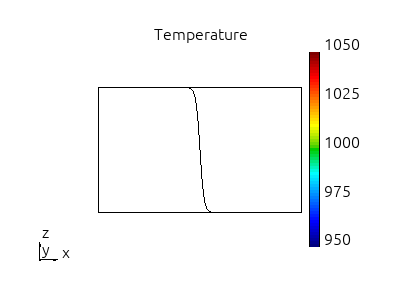
\includegraphics[width=0.5\textwidth]{figs/temperature_p51DT1000.png} &
      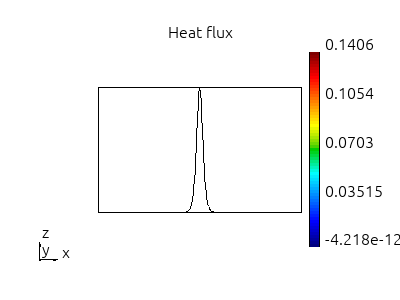
\includegraphics[width=0.5\textwidth]{figs/hflux_p51DT1000.png} \\
      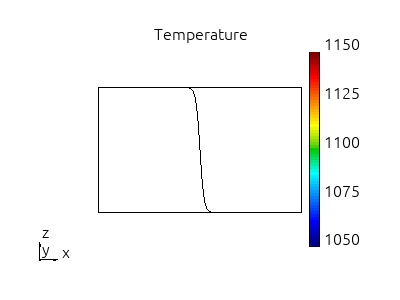
\includegraphics[width=0.5\textwidth]{figs/temperature_p51DT1100.png} &
      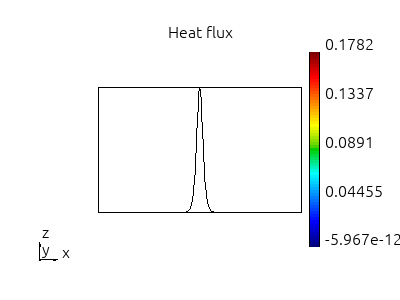
\includegraphics[width=0.5\textwidth]{figs/hflux_p51DT1100.png}
    \end{tabular}
  \caption{
    Problem 5 - AWBS nonlinearity check.
  }
  \end{center}
  \label{fig:p51D_AWBS_nonlinearity}
\end{figure}
\clearpage
\subsection{Analysis of nonlocality}\label{sec:NonlocalityAnalysis}
\begin{figure}[tbh]
  \begin{center}
    \begin{tabular}{cc}
      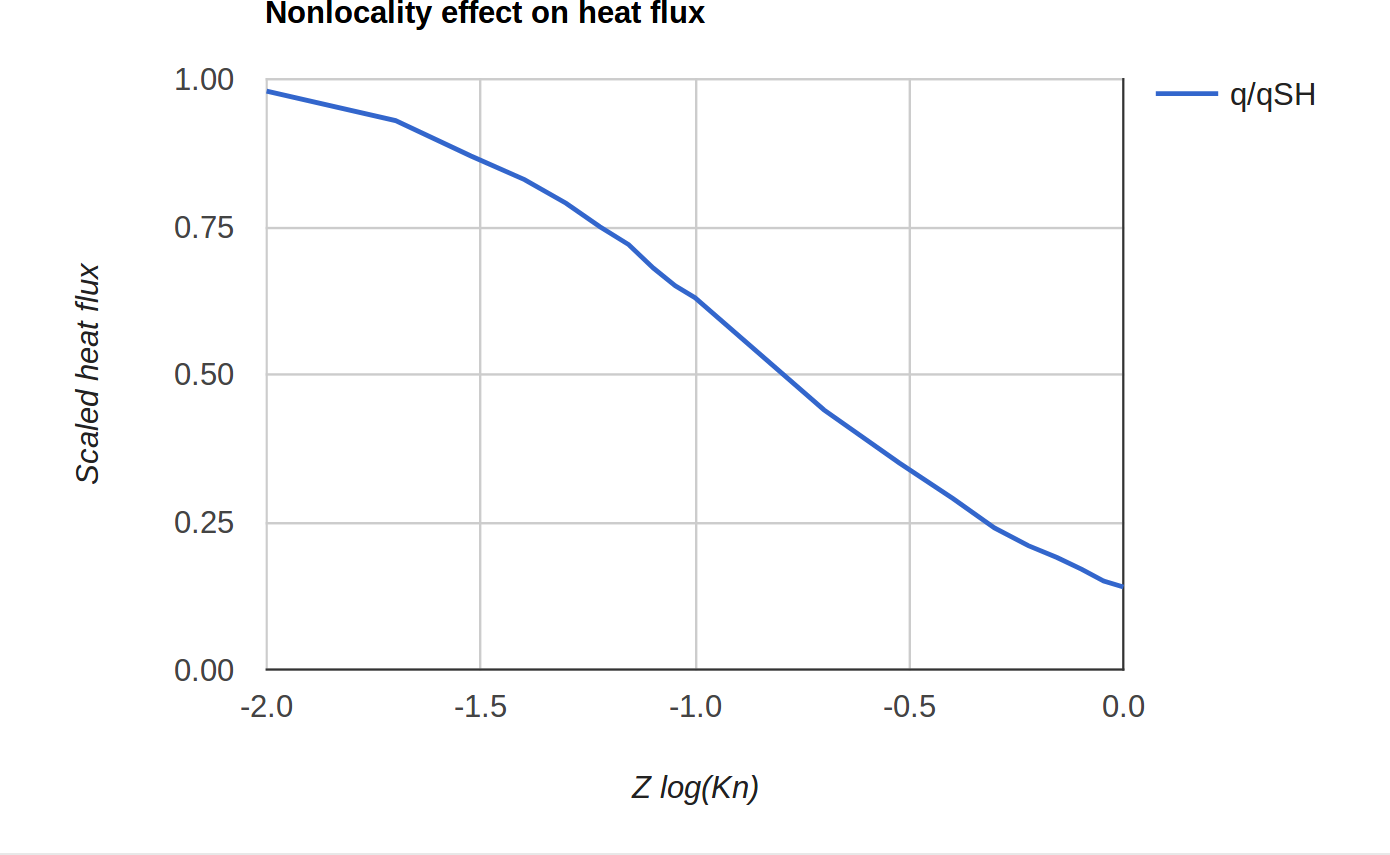
\includegraphics[width=0.45\textwidth]{Nonlocality_analysis_woutE.png} &
	  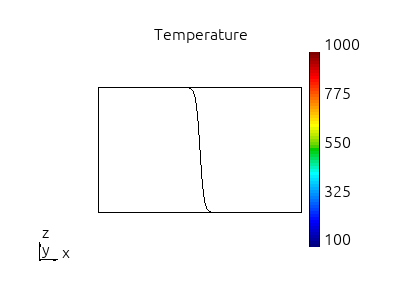
\includegraphics[width=0.45\textwidth]{figs/temperature_p51DNonlocAnal.png} 
    \end{tabular}
  \caption{
    M1-AWBS model. Left: The~maximum of computed flux normalized with respect 
	to the~value of SH flux. E field effect is not included.  
	Right: Corresponding temperature profile. Density and ionization 
	(scattering on Z = 100 included) have been kept constant.
  }
  \end{center}
  \label{fig:nonlocality_analysis}
\end{figure}

\begin{figure}[tbh]
  \begin{center}
    \begin{tabular}{ccc}
      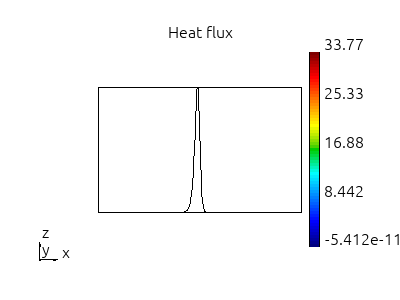
\includegraphics[width=0.3\textwidth]{figs/hflux_p51DKn1e-3.png} &
	  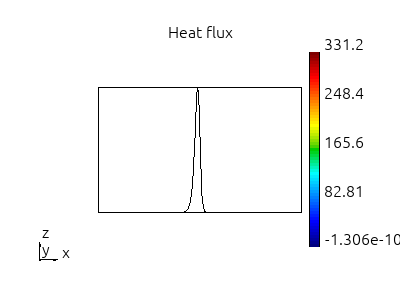
\includegraphics[width=0.3\textwidth]{figs/hflux_p51DKn1e-2.png} & 
      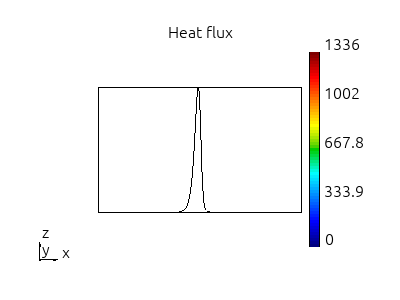
\includegraphics[width=0.3\textwidth]{figs/hflux_p51DKn5e-2.png} \\
	  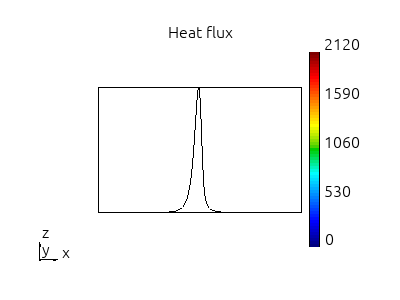
\includegraphics[width=0.3\textwidth]{figs/hflux_p51DKn1e-1.png} &
      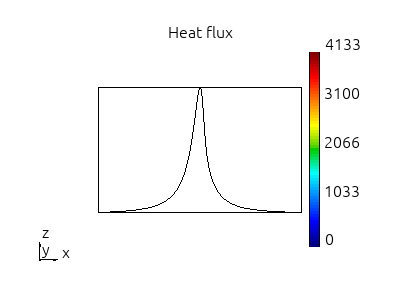
\includegraphics[width=0.3\textwidth]{figs/hflux_p51DKn5e-1.png} &
	  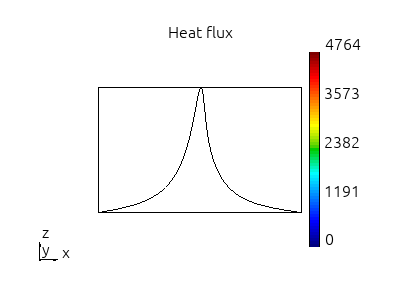
\includegraphics[width=0.3\textwidth]{figs/hflux_p51DKn1e0.png} 
    \end{tabular}
  \caption{
    Heat flux calculated by M1-AWBS model. Figures in left-right top-bottom 
	order correspond to Kn = 0.001, 0.01, 0.05, 0.1, 0.5, 1.0. 
	E field effect is not included.  
	Density and ionization (Z = 100) have been kept constant.
  }
  \end{center}
  \label{fig:nonlocality_analysis_fluxes}
\end{figure}

Some observations:
\begin{itemize}
  \item Our calculated distribution function is thermalized, 
  i.e. $f_0 = \fM$.
  \item With added scattering we also obtain the correct value of calculated 
  heat flux, i.e. $q = q_{SH}$, nevertheless, this works with no E field.
  \item The E field effect is implemented. When tested with the analytic 
  formula $E_{SH} = \vth^2(\nabla ne /ne + 5/2 nabla T/T)$ 
  (we consider Z=100),
  the corresponding flux reduction due to E field is also correct 
  (flux is reduced to 30$\%$ of its E=0 value).
  \item However, the $E_{SH}$ does not work under any condition, 
  i.e. it exhibits some extra dependence on temperature.
\end{itemize}

\begin{figure}[tbh]
  \begin{center}
    \begin{tabular}{cc}
      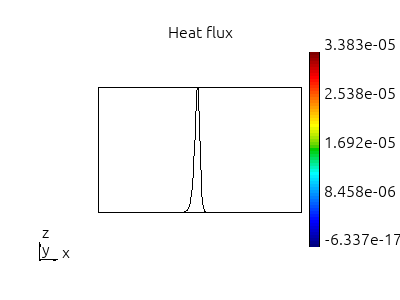
\includegraphics[width=0.5\textwidth]{figs/hflux_p51DKn1e-9.png} &
      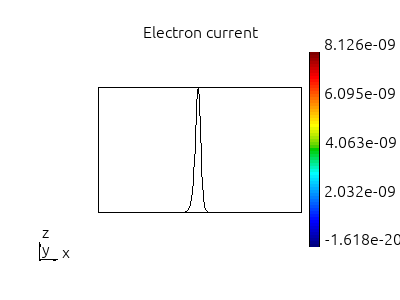
\includegraphics[width=0.5\textwidth]{figs/jcurrent_p51DKn1e-9.png} \\
	  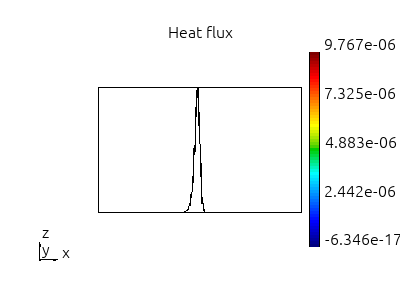
\includegraphics[width=0.5\textwidth]{figs/hflux_p51DKn1e-9Efield.png} &
      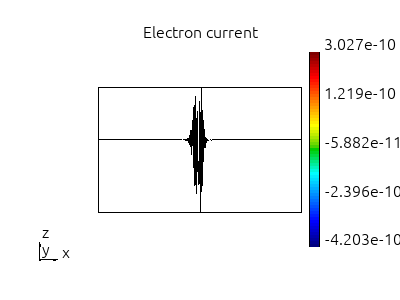
\includegraphics[width=0.5\textwidth]{figs/jcurrent_p51DKn1e-9Efield.png}  
    \end{tabular}
  \caption{
    Preliminary results with respect to the E field effect. 
	The SH analytic formula for E field leads to the~corresponding current 
	reduction ($j \approx 0$). The corresponding heat flux is reduced 
	$\approx$ by 70 $\%$, exactly as predicted. Nevertheless, the~formula 
	exhibits some dependence on temperature (not on its gradient and also not
	on the~mean free path).
  }
  \end{center}
  \label{fig:p41D_rho_T}
\end{figure}
\clearpage

\newcommand{\psize}{0.45}
\begin{figure}[tbh]
  \begin{center}
    \begin{tabular}{cc}
      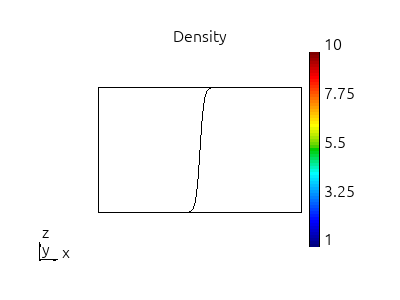
\includegraphics[width=0.5\textwidth]{figs/density_p41D.png} &
      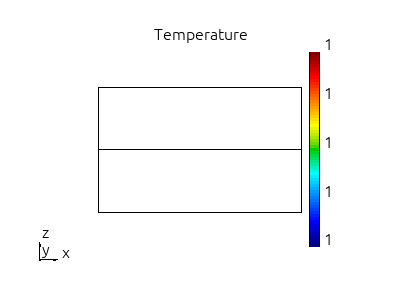
\includegraphics[width=0.5\textwidth]{figs/temperature_p41D.png}
    \end{tabular}
  \caption{
    Problem 4 background.
  }
  \end{center}
  \label{fig:p41D_rho_T}
\end{figure}

\begin{figure}[tbh]
  \begin{center}
    \begin{tabular}{cc}
      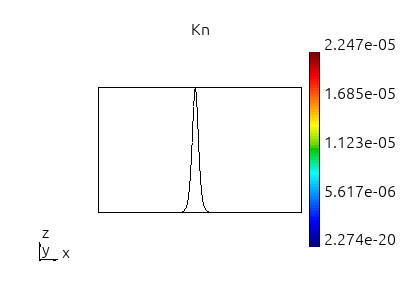
\includegraphics[width=\psize\textwidth]{figs/Kn_p41D1e6.png} &
      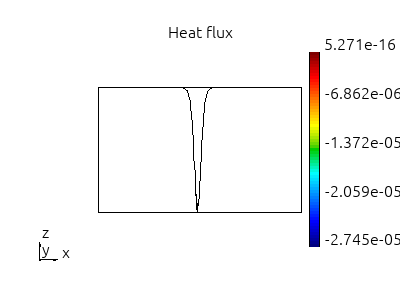
\includegraphics[width=\psize\textwidth]{figs/hflux_p41D1e6.png} \\
      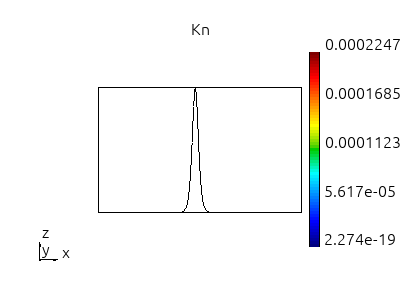
\includegraphics[width=\psize\textwidth]{figs/Kn_p41D1e5.png} &
      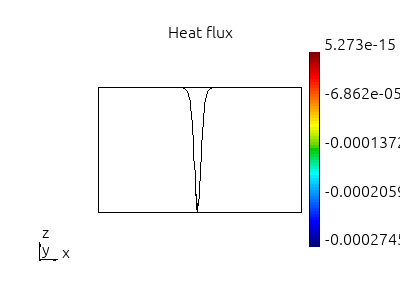
\includegraphics[width=\psize\textwidth]{figs/hflux_p41D1e5.png} \\
      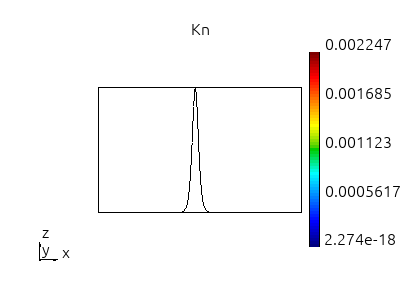
\includegraphics[width=\psize\textwidth]{figs/Kn_p41D1e4.png} &
      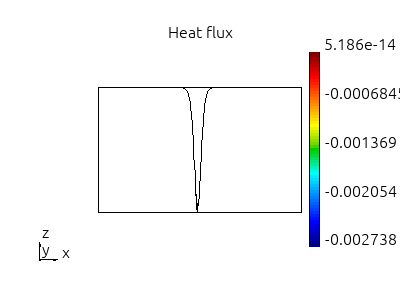
\includegraphics[width=\psize\textwidth]{figs/hflux_p41D1e4.png} \\
      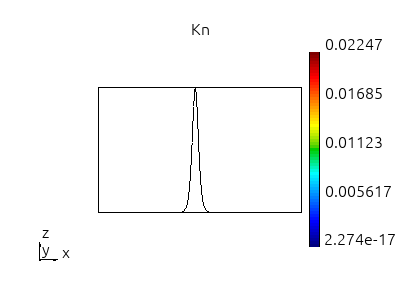
\includegraphics[width=\psize\textwidth]{figs/Kn_p41D1e3.png} &
      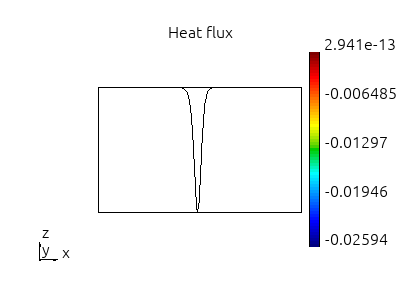
\includegraphics[width=\psize\textwidth]{figs/hflux_p41D1e3.png} \\
      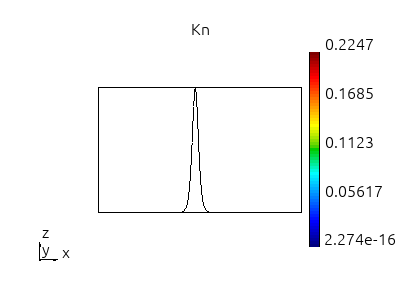
\includegraphics[width=\psize\textwidth]{figs/Kn_p41D1e2.png} &
      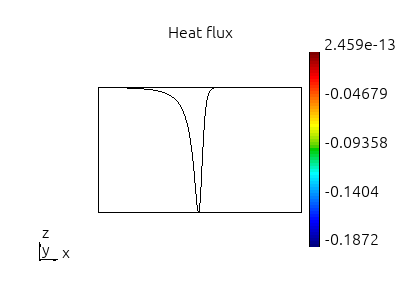
\includegraphics[width=\psize\textwidth]{figs/hflux_p41D1e2.png} 
    \end{tabular}
  \caption{
    Problem 4 transport.
  }
  \end{center}
  \label{fig:p4_Kn_hflux}
\end{figure}

\begin{figure}[tbh]
  \begin{center}
    \begin{tabular}{cc}
      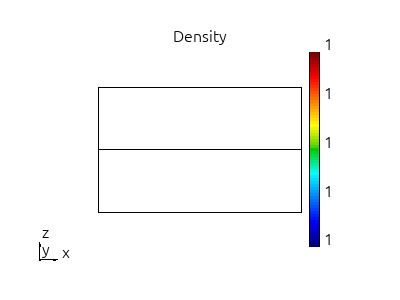
\includegraphics[width=0.5\textwidth]{figs/density_p51D.png} &
      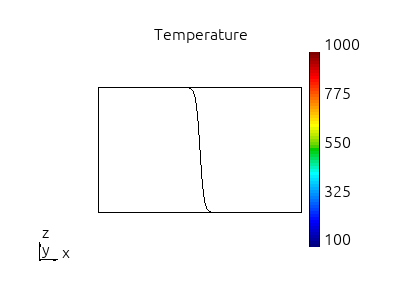
\includegraphics[width=0.5\textwidth]{figs/temperature_p51D.png}
    \end{tabular}
  \caption{
    %Problem 5 background.
	VFP-paper corresponding simulations, ion background density and 
	temperature.
  }
  \end{center}
  \label{fig:p51D_rho_T}
\end{figure}

\begin{figure}[tbh]
  \begin{center}
    \begin{tabular}{cc}
      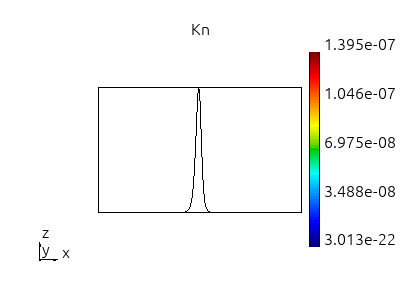
\includegraphics[width=\psize\textwidth]{figs/Kn_p51D1e14.png} &
      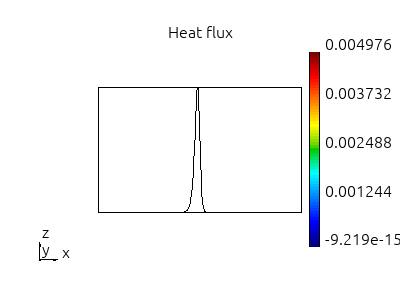
\includegraphics[width=\psize\textwidth]{figs/hflux_p51D1e14.png} \\
      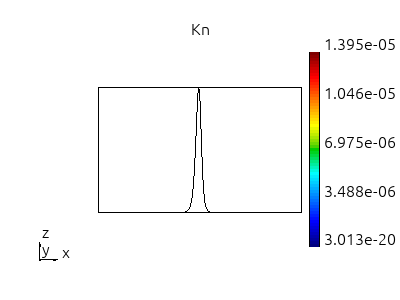
\includegraphics[width=\psize\textwidth]{figs/Kn_p51D1e12.png} &
      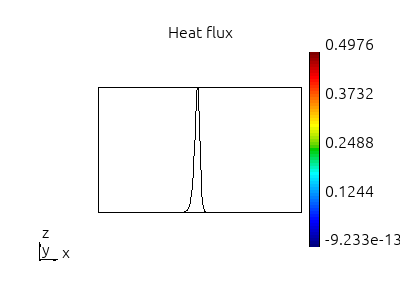
\includegraphics[width=\psize\textwidth]{figs/hflux_p51D1e12.png} \\
      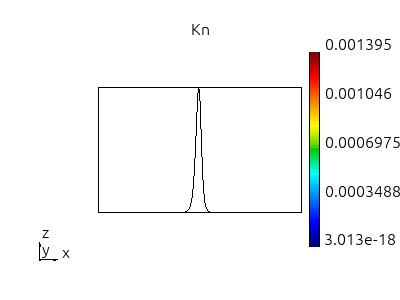
\includegraphics[width=\psize\textwidth]{figs/Kn_p51D1e10.png} &
      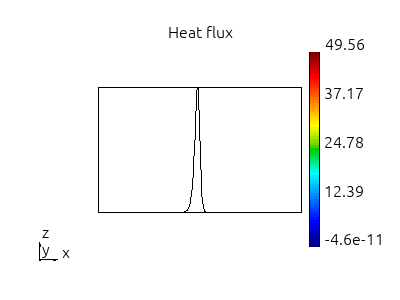
\includegraphics[width=\psize\textwidth]{figs/hflux_p51D1e10.png} \\
      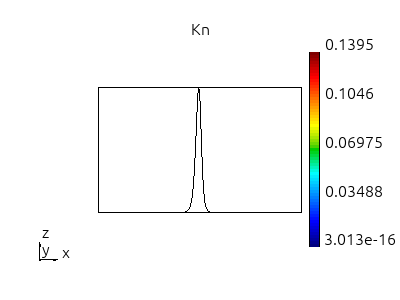
\includegraphics[width=\psize\textwidth]{figs/Kn_p51D1e8.png} &
      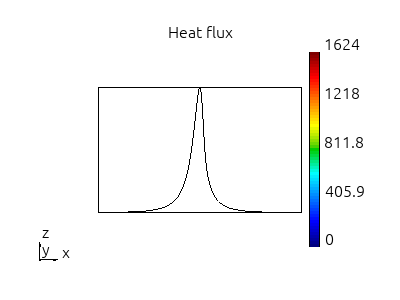
\includegraphics[width=\psize\textwidth]{figs/hflux_p51D1e8.png} 
	  %\\
      %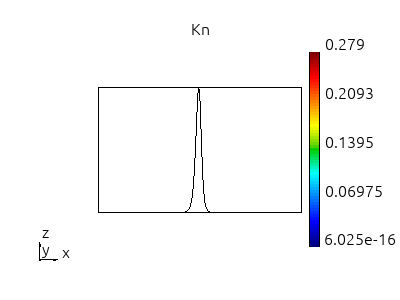
\includegraphics[width=\psize\textwidth]{figs/Kn_p51D5e7.png} &
      %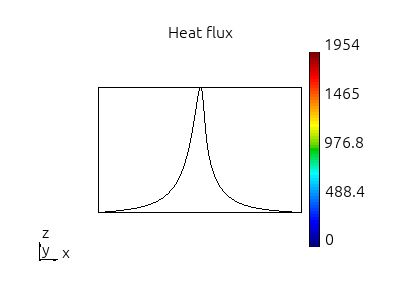
\includegraphics[width=\psize\textwidth]{figs/hflux_p51D5e7.png} 
    \end{tabular}
  \caption{
    %Problem 5 transport.
	VFP-paper corresponding simulations, Kn spans the interval 
	$(\approx 10^{-7}, \approx 10^{-1})$ where flux goes from diffusive to
	highly nonlocal.
  }
  \end{center}
  \label{fig:p5_Kn_hflux}
\end{figure}

\begin{figure}[tbh]
  \begin{center}
    \begin{tabular}{cc}
      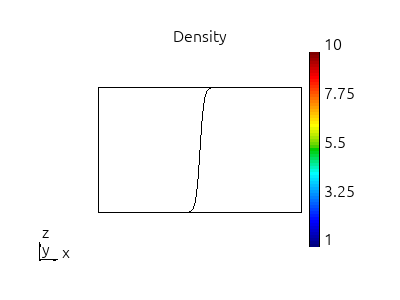
\includegraphics[width=0.5\textwidth]{figs/density_p61D.png} &
      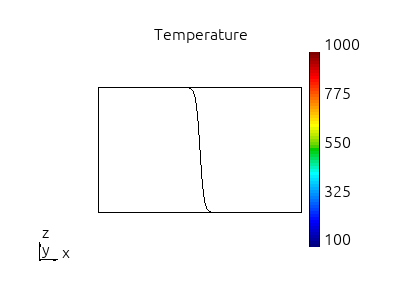
\includegraphics[width=0.5\textwidth]{figs/temperature_p61D.png}
    \end{tabular}
  \caption{
    Problem 6 background.
  }
  \end{center}
  \label{fig:p51D_rho_T}
\end{figure}

\begin{figure}[tbh]
  \begin{center}
    \begin{tabular}{cc}
      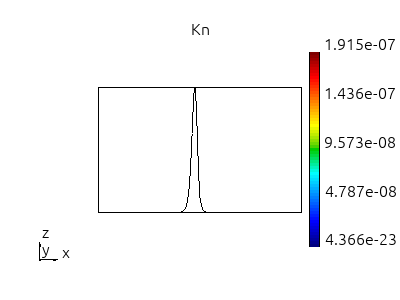
\includegraphics[width=\psize\textwidth]{figs/Kn_p61D1e14.png} &
      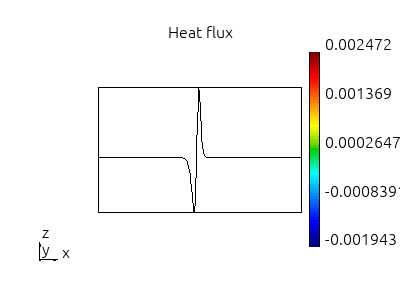
\includegraphics[width=\psize\textwidth]{figs/hflux_p61D1e14.png} \\
      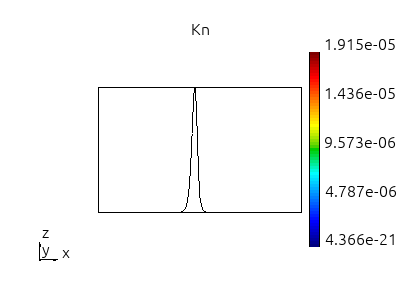
\includegraphics[width=\psize\textwidth]{figs/Kn_p61D1e12.png} &
      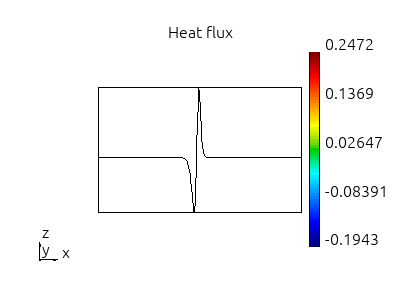
\includegraphics[width=\psize\textwidth]{figs/hflux_p61D1e12.png} \\
      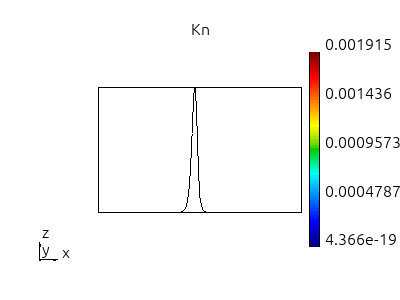
\includegraphics[width=\psize\textwidth]{figs/Kn_p61D1e10.png} &
      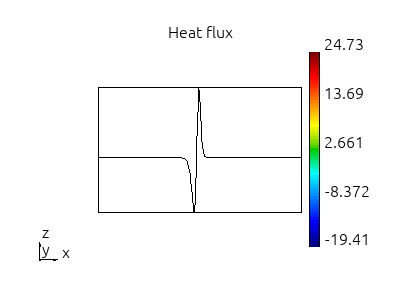
\includegraphics[width=\psize\textwidth]{figs/hflux_p61D1e10.png} \\
      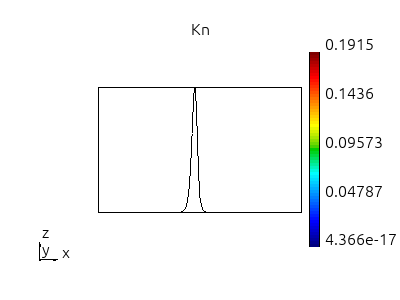
\includegraphics[width=\psize\textwidth]{figs/Kn_p61D1e8.png} &
      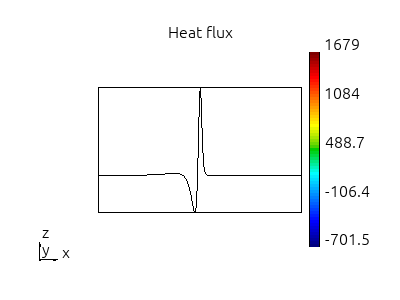
\includegraphics[width=\psize\textwidth]{figs/hflux_p61D1e8.png} \\
      \includegraphics[width=\psize\textwidth]{figs/Kn_p61D5e7.png} &
      \includegraphics[width=\psize\textwidth]{figs/hflux_p61D5e7.png} 
    \end{tabular}
  \caption{
    Problem 6 transport.
  }
  \end{center}
  \label{fig:p6_Kn_hflux}
\end{figure}

\begin{figure}[tbh]
  \begin{center}
    \begin{tabular}{cc}
      \includegraphics[width=0.5\textwidth]{figs/density_p71D.png} &
      \includegraphics[width=0.5\textwidth]{figs/temperature_p71D.png}
    \end{tabular}
  \caption{
    Problem 7 background.
  }
  \end{center}
  \label{fig:p71D_rho_T}
\end{figure}

\begin{figure}[tbh]
  \begin{center}
    \begin{tabular}{cc}
      \includegraphics[width=\psize\textwidth]{figs/Kn_p71D1e14.png} &
      \includegraphics[width=\psize\textwidth]{figs/hflux_p71D1e14.png} \\
      \includegraphics[width=\psize\textwidth]{figs/Kn_p71D1e12.png} &
      \includegraphics[width=\psize\textwidth]{figs/hflux_p71D1e12.png} \\
      \includegraphics[width=\psize\textwidth]{figs/Kn_p71D1e10.png} &
      \includegraphics[width=\psize\textwidth]{figs/hflux_p71D1e10.png} \\
      \includegraphics[width=\psize\textwidth]{figs/Kn_p71D1e8.png} &
      \includegraphics[width=\psize\textwidth]{figs/hflux_p71D1e8.png} \\
      \includegraphics[width=\psize\textwidth]{figs/Kn_p71D5e7.png} &
      \includegraphics[width=\psize\textwidth]{figs/hflux_p71D5e7.png} 
    \end{tabular}
  \caption{
    Problem 7 transport.
  }
  \end{center}
  \label{fig:p7_Kn_hflux}
\end{figure}

\begin{figure}[tbh]
  \begin{center}
    \begin{tabular}{cc}
      \includegraphics[width=0.5\textwidth]{figs/density_p71D.png} &
      \includegraphics[width=0.5\textwidth]{figs/temperature_p71D.png} \\
      \includegraphics[width=0.5\textwidth]{figs/density_p72D.png} &
      \includegraphics[width=0.5\textwidth]{figs/temperature_p72D.png} \\
      \includegraphics[width=0.5\textwidth]{figs/density_p73D.png} &
      \includegraphics[width=0.5\textwidth]{figs/temperature_p73D.png} 
    \end{tabular}
  \caption{
    Problem 7 1D/2D/3D background.
  }
  \end{center}
  \label{fig:p71D_rho_T}
\end{figure}

\renewcommand{\psize}{0.33}
\begin{figure}[tbh]
  \begin{center}
    \begin{tabular}{ccc}
      \includegraphics[width=\psize\textwidth]{figs/Kn_p71D1e12.png} &
      \includegraphics[width=\psize\textwidth]{figs/Kn_p71D1e10.png} &
      \includegraphics[width=\psize\textwidth]{figs/Kn_p71D1e8.png} \\
	  \includegraphics[width=\psize\textwidth]{figs/hflux_p71D1e12.png} &
      \includegraphics[width=\psize\textwidth]{figs/hflux_p71D1e10.png} &
      \includegraphics[width=\psize\textwidth]{figs/hflux_p71D1e8.png} \\
	  \includegraphics[width=\psize\textwidth]{figs/hflux_p72D1e12.png} &
      \includegraphics[width=\psize\textwidth]{figs/hflux_p72D1e10.png} &
      \includegraphics[width=\psize\textwidth]{figs/hflux_p72D1e8.png} \\
	  \includegraphics[width=\psize\textwidth]{figs/hflux_p73D1e12.png} &
      \includegraphics[width=\psize\textwidth]{figs/hflux_p73D1e10.png} &
      \includegraphics[width=\psize\textwidth]{figs/hflux_p73D1e8.png} \\
    \end{tabular}
  \caption{
    Problem 7 1D/2D/3D transport.
  }
  \end{center}
  \label{fig:p7_Kn_hflux}
\end{figure}

\begin{figure}[tbh]
  \begin{center}
    \begin{tabular}{c}
      \includegraphics[width=1.0\textwidth]{M1Sedov1D2D3D.png} \\
      \includegraphics[width=1.0\textwidth]{M1_physical_analysis.png}
    \end{tabular}
  \caption{
  Sedov blast in 1D/2D/3D from $\delta$ function hot spot. 
  Shock propagates from left to right. Top raw corresponds to 1D 
  (8858 energy groups) - 
  left: density profile, right: temperature 
  (decreasing from the~original hot spot with low temperature in compressed 
  plasma), center: heat flux with its maximum on the~start of increase 
  in density decreasing while approaching the~shock 
  (NOTICE non-zero flux ahead of the~shock). 
  Middle raw corresponds to 2D (4348 energy groups) - 
  left: density, center: heat flux, right: temperature.
  Bottom raw corresponds to 3D (10030 energy groups) - 
  left: density, center: heat flux, right: temperature. 
  }
  \end{center}
  \label{fig:expl1D2D3D}
\end{figure}

\subsection{Implicit fully-discrete scheme}\label{sec:impl_fullydiscrete_scheme}
In order to formulate a~fully-discrete scheme leaning on an~implicit 
discretization of velocity, the~equations \eqref{eq:semiM1hosf0} and 
\eqref{eq:semiM1hosf1} can be expressed with matrices as
\begin{eqnarray}
  \matr{M}_0 \cdot \pdv{\vfzero}{\vmag}  
  &=& 
  \matr{D}_0 \cdot \fone
  + \matr{E}_0^1 \cdot \pdv{\fone}{\vmag} + \matr{E}_0^2 \cdot \fone
  + \matr{M}_0 \cdot \pdv{\vect{\fM}}{\vmag} ,  
  \nonumber\\
  \matr{M}_1 \cdot \pdv{\fone}{\vmag}  
  &=& 
  - \matr{D}_1 \cdot \vfzero 
  + \matr{E}_1^1 \cdot \pdv{\vfzero}{\vmag}
  + \matr{E}_1^2 \cdot \vfzero
  + \matr{B} \cdot \fone
  + \matr{M}^t_1 \cdot \fone ,
  \nonumber
\end{eqnarray}

\begin{eqnarray}
  \ddv{\vfzero}{\vmag}  
  &=& 
  \matr{M}_0^{-1} \cdot \left(\matr{D}_0 + \matr{E}_0^2 \right) 
  \cdot \left(\fone^n + \Delta \vmag \ddv{\fone}{\vmag} \right)
  + \matr{M}_0^{-1} \cdot \matr{E}_0^1 \cdot \ddv{\fone}{\vmag} \nonumber\\
  && + \pdv{\vect{\fM}}{\vmag} ,  
  \nonumber\\
  \matr{M}_1 \cdot \ddv{\fone}{\vmag}  
  &=& 
  \left( \matr{E}_1^2 - \matr{D}_1 \right) 
  \cdot \left(\vfzero^n + \Delta\vmag \ddv{\vfzero}{\vmag} \right) 
  + \matr{E}_1^1 \cdot \ddv{\vfzero}{\vmag} \nonumber\\
  && + \left( \matr{B} + \matr{M}^t_1 \right)  
  \cdot \left(\fone^n + \Delta \vmag \ddv{\fone}{\vmag} \right) ,
  \nonumber
\end{eqnarray}

\begin{eqnarray}
  \ddv{\vfzero}{\vmag}  
  &=& 
  \matr{\tilde{A}}_0 \cdot \ddv{\fone}{\vmag}
  + \vect{b}_0\left(\fone^n, \pdv{\vect{\fM}}{\vmag}\right) ,  
  \label{eq:df0dv} \\
  \left( \matr{M}_1 
  - \Delta \vmag \left( \matr{B} + \matr{M}^t_1 \right) \right) 
  \cdot \ddv{\fone}{\vmag}  
  &=& 
  \matr{\tilde{A}}_1 \cdot \ddv{\vfzero}{\vmag}  
  + \vect{b}_1 \left( \fone^n, \vfzero^n \right) , 
  \label{eq:df1dvdf0dv}
\end{eqnarray}

\begin{equation}
  \left( \matr{M}_1 
  - \Delta \vmag \left( \matr{B} + \matr{M}^t_1 \right) 
  - \matr{\tilde{A}}_1 \cdot \matr{\tilde{A}}_0 \right) 
  \cdot \ddv{\fone}{\vmag}  
  = 
  \matr{\tilde{A}}_1 
  \cdot \vect{b}_0 + \vect{b}_1 , 
  %\matr{\tilde{A}}_1 
  %\cdot \vect{b}_0\left(\fone^n, \pdv{\vect{\fM}}{\vmag}\right)
  %+ \vect{b}_1 \left( \fone^n, \vfzero^n \right)~, 
  \label{eq:df1dv}
\end{equation}

\cite{Dobrev_Kolev_Rieben-High-order_curvilinear_finite_element_methods_for_Lagrangian_hydrodynamics}

%---------------------------------------------------------------------
%---------------------------------------------------------------------
%---------------------------------------------------------------------
\section*{References}
\bibliography{NTH}


%---------------------------------------------------------------------
%---------------------------------------------------------------------


\end{document}

%---------------------------------------------------------------------
%---------------------------------------------------------------------
